\subsection{Развертывание программного средства}
\label{sec:design:deployment}

После выявления, а также завершения проектирования всех компонентов программного средства появляется вопрос о планировании развертывания всей системы. 
Необходимо составить описание требуемых аппа-ратно-программных комплексов, которые понадобятся для работы приложения. 
Для этих целей и составляется диаграмма развертывания. 

Данная диаграмма представлена на рисунке~\ref{fig:design:deployment:diagram}. Она отражает следующие особенности развертывания:

\begin{itemize}
	\item На узле конечного устройства в качестве среды выполнения перечислен список операционных систем, поддерживаемых клиентским приложением и программой для создания пакетов вопросов.
	\item Предполагается, что пользовательское конечное устройство зна\-чи\-те\-льно удалено от серверов программной системы, доступ осуществляется через сеть Интернет, что и упрощенно показано на диаграмме.
\end{itemize}

Таким образом, после развертывания программного средства пользователи могут уже использовать клиент приложения для организации и проведения викторин.

\begin{figure}[!ht]
\centering
    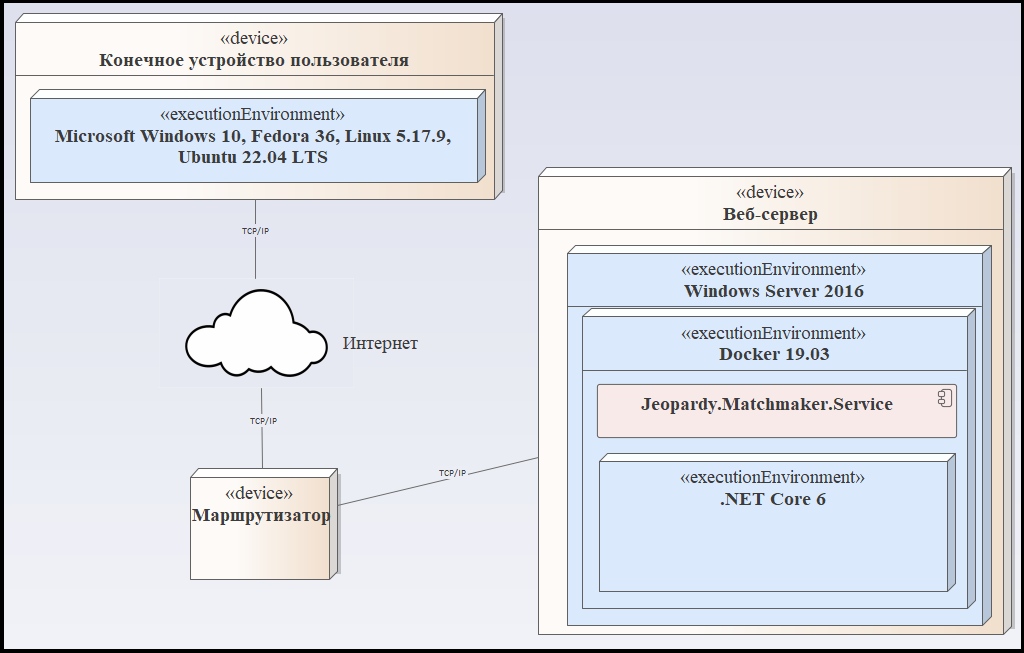
\includegraphics[scale=0.6]{attachments/deploy.png}
    \caption{Диаграмма развертывания ПС}
    \label{fig:design:deployment:diagram}
\end{figure}